\chapter{Approach}
The author in \cite{b6} proposes a step approach to carry out desynchronization attacks. Figure \ref{fig:Phases} shows the phases of a desynchronization attack or request smuggling. Before explaining each of the phases in request smuggling, we need to observe that there are four possible configurations between the systems:
\begin{itemize}
	\item \textbf{CL.CL : } Both the frontend and backend servers use \textsc{Content-Length} header. As we have already seen, this configuration doesn't help in realizing attacks on practical modern systems. 
	\item \textbf{CL.TE : } Frontend server uses \textsc{Content-Length} header field and Backend server uses \textsc{Transfer-Encoding} header field. 
	\item \textbf{TE.CL : } Frontend server uses \textsc{Transfer-Encoding} header field and Backend server uses \textsc{Content-Length} header field.
	\item \textbf{TE.TE : } Both the frontend and backend servers use \textsc{Transfer-Encoding} header field.
\end{itemize}
\begin{figure}
	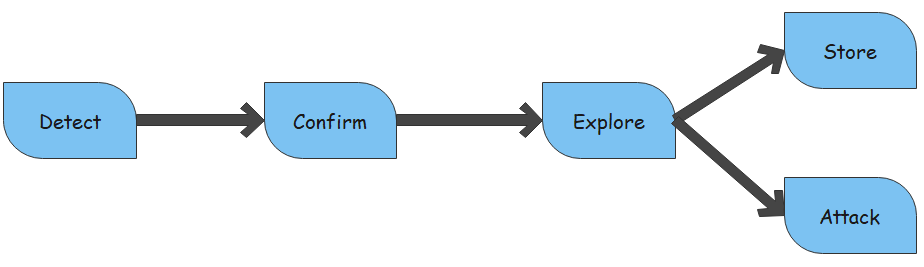
\includegraphics[width=14cm]{images/Phases}
	\caption{Phases of request smuggling}
	\label{fig:Phases}
\end{figure}
We will now look at each of the phases in detail:
\section{Detect}
The first step is to detect when a server will be vulnerable to desynchronization. A simple method here is to send a request with malicious data and poison the backend. Subsequent back to back requests are then sent to the same backend server. If the subsequent requests get an unexpected or erroneous response, we can assume that the response was due to the malicious prefix sent with the first request.  \\
However this technique isn't as simple as it looks and has a major drawback. When we try to detect desynchronization vulnerabilities in a website with a live traffic, there are numerous requests coming from many different users. If there is a normal user's request between our first malicious request and the subsequent follow up requests we send, it causes an error to the normal user and doesn't affect the follow up requests. Hence we cannot detect the vulnerability as we will not be able to observe the responses. \\
To tackle this problem, the author in \cite{b6} proposes an approach which uses server time-outs to the attacker's advantage. The configuration \textbf{CL.CL} and \textbf{TE.TE} cannot be used here for our advantage. However, \textbf{CL.TE} and \textbf{TE.CL} can be used. \\

\begin{figure}
	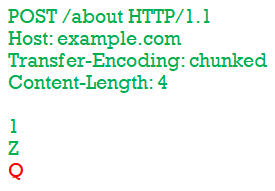
\includegraphics{images/CL.TE}
	\caption{CL.TE}
	\label{fig:CL.TE}
\end{figure}

\begin{figure}
	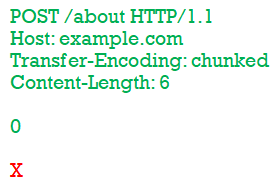
\includegraphics{images/TE.CL}
	\caption{TE.CL}
	\label{fig:TE.CL}
\end{figure}

\subsection{Case Study for \textit{Detect} phase}
Consider the example for \textbf{CL.TE} in figure \ref{fig:CL.TE}(Referenced from \cite{b6}). As \textcolor{myred}{Q} is not a valid chunk size, the frontend will forward only the information highlighted in \textcolor{mygreen}{green} and the backend will timeout waiting for next valid chunk size. \\
Consider another example for \textbf{TE.CL} in figure \ref{fig:TE.CL}(Referenced from \cite{b6}). In this request, \textcolor{mygreen}{0} is explicitly placed to force the server into considering it as the \textit{terminating chunk}. As a result, the server will timeout waiting for \textcolor{myred}{X}.\\
These observable delays are sufficient to infer that the system has a vulnerability for request smuggling.\\

\section{Confirm}
Once we are sure that a system is vulnerable for request smuggling, we need to confirm the same with the help of responses that serve as visible proofs. The technique to get such confirmation is by poisoning the backend socket. One the follow-up requests we send will fall victim to the earlier poisoning and will return a response to visibly prove that the vulnerability is present. One hindrance here is disconnection. If the first request causes an error, the backend system may have been designed to drop the connection and associated buffers. Such a disconnection will fail the attack. This can be avoided by targeting backend server endpoints which accept POST requests. 
\subsection{Case Study for \textit{Confirm} phase}
\textit{Referenced from \cite{b6}}\\
\begin{figure}
	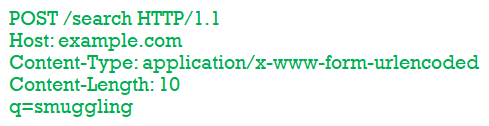
\includegraphics{images/Confirm_Request}
	\caption{Confirm - Target Request}
	\label{fig:Confirm_Request}
\end{figure}
If the target request looks as in figure \ref{fig:Confirm_Request}, then two types of socket poisoning are possible:
\begin{itemize}
	\item \textbf{CL.TE : } The request created for CL.TE poisoning is basically aiming to force a 404 response to the follow-up victim request. Figure \ref{fig:Confirm-CL.TE Poisoning}  
	\begin{figure}
		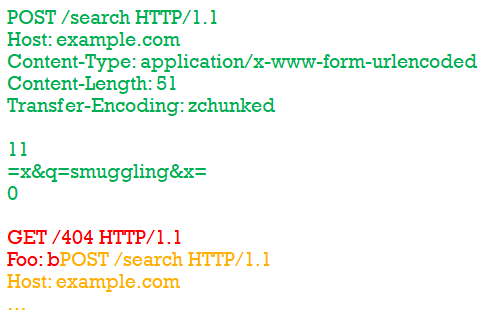
\includegraphics{images/Confirm_CL.TE}
		\caption{Confirm - CL.TE Poisoning}
		\label{fig:Confirm-CL.TE Poisoning}
	\end{figure}
	\item \textbf{TE.CL : } This is similar to CL.TE but the attacker needs to specify all the headers and ensure that the length of the malicious prefix is larger than the body. Figure \ref{fig:Confirm-TE.CL Poisoning}
	\begin{figure}
		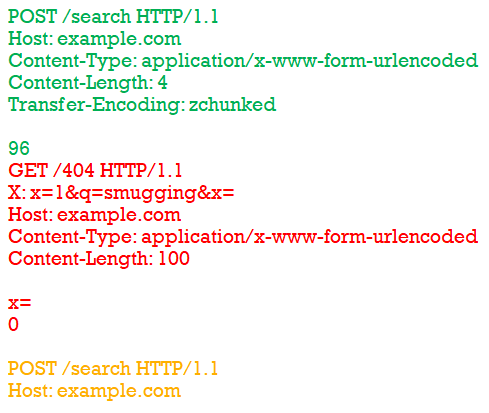
\includegraphics{images/Confirm_TE.CL}
		\caption{Confirm - TE.CL Poisoning}
		\label{fig:Confirm-TE.CL Poisoning}
	\end{figure}
\end{itemize}

\section{Explore}
Once we have established the fact that a target system is vulnerable for request smuggling attacks and the servers can be poisoned, we have to explore the ways in which an attack can be carried out. Explore phase aims to gather sensitive information which will help in attacking the target system. \\
There are several HTTP request headers which are often re-written by the frontend servers while transmitting the request. Though we try to change these headers manually, the frontend still re-writes these headers. For example, X-Forwarded-Host and X-Forwarded-For. This kind of configuration usually makes it difficult to by-pass such re-writes because the smuggled request may be missing these headers and can cause the system to exhibit unexpected behaviour. \\
One method to navigate across such header re-writes is to gradually gain visibility into these hidden headers by sending numerous investigative requests, observing the responses and further modifying the requests everytime before re-sending. This method is followed until the response reveals some information about the hidden headers, which we can use for our advantage. Once the hidden headers are revealed, we can modify our request to include these headers and further carryout attacks on the system. 
\subsection{Case Study for \textit{Explore} phase}
One simple example (as referenced from \cite{b6}) to demonstrate this is to explore a page in the target application which reflects a POST parameter. The smuggled request is modified accordingly by placing the reflected parameter at the last and increasing the \textsc{Content-length}. The modified request can now be smuggled. Figure \ref{fig:Explore_Request} shows one such example request.\\ 
\begin{figure}
	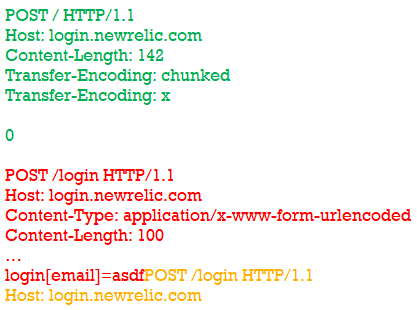
\includegraphics{images/Explore_Request}
	\caption{Explore - Request}
	\label{fig:Explore_Request}
\end{figure}
The follow-up request will be re-written by the frontend server before it encounters the $login[email]$ parameter. When the response is received, all the internal headers are revealed. 
The response to the request in figure \ref{fig:Explore_Request} can be as follows:
\begin{verbatim}
Please ensure that your email and password are correct.
<input id="email" value="asdfPOST /login HTTP/1.1
Host: login.newrelic.com
X-Forwarded-For: 81.139.39.150
X-Forwarded-Proto: https
X-TLS-Bits: 128
X-TLS-Cipher: ECDHE-RSA-AES128-GCM-SHA256
X-TLS-Version: TLSv1.2
x-nr-external-service: external
\end{verbatim}
Increasing the \textsc{Content-Length} header can reveal more and more information, until the entire victim request is parsed. 

\section{Store}
Once we explore the possible methods of poisoning the servers, we have two possibilities. One is to attack the victim or to store their data. In the store phase, we mainly aim to store the data revealed by the response to a victim's request. Once the server is poisoned with the malicious prefix we introduce, it gets appended to the next request. If a normal user (victim) sends this next request, their data can be stored and then we can make the application reveal their sensitive information. \\
For this method to work, the application needs to support some kind of data storage. If this is supported, the malicious prefix we send can be carefully crafted to contain a storage request. When this is appended to victim's request, it is possible to force the application to store the victim's information such as cookies/headers. 
\subsection{Case Study for \textit{Store} phase}
Figure \ref{fig:Store_Request} referenced from \cite{b6} demonstrates an example of storing victim's information.
\begin{figure}
	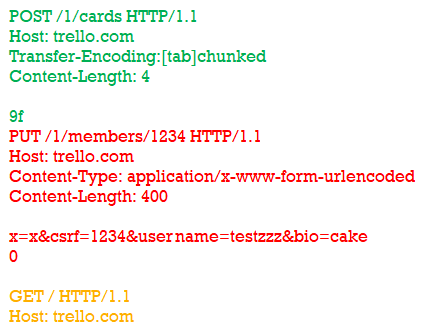
\includegraphics{images/Store_Request}
	\caption{Store - Request}
	\label{fig:Store_Request}
\end{figure}
The malicious prefix was crafted to target the Trello's profile-edit endpoint and was designed to store a victim's information on a test account in Trello.\\
\begin{figure}
	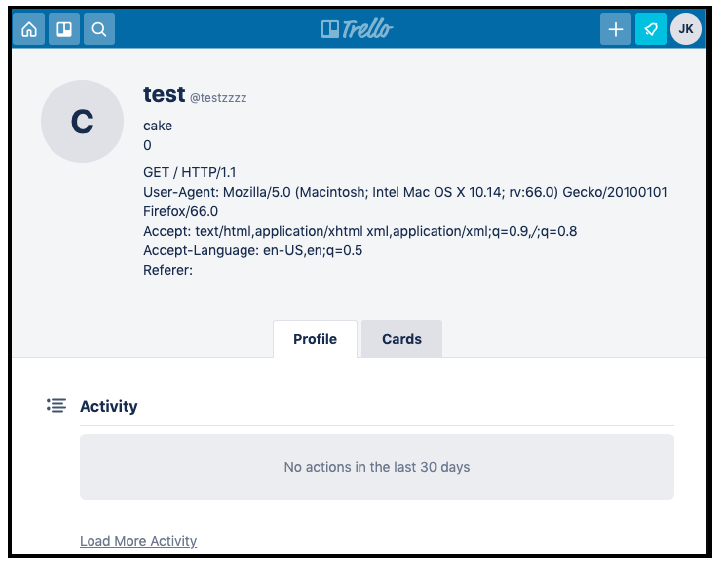
\includegraphics[width=14cm]{images/Store_Response}
	\caption{Store - Response}
	\label{fig:Store_Response}
\end{figure}
When the prefix got appended to the victim's request, their cookies and headers were routed to the test account and the same were displayed in that account. See figure \ref{fig:Store_Response} (Referenced from \cite{b6})\\

\section{Attack}
After exploring the poisoning options, another further option is to directly carry out the attack on the victims by triggering a harmful response. \\
Two primary methods for attacks are :
\begin{itemize}
	\item Trigger harmful response : Send malicious prefix that can 'attack', wait for the victim's request to get appended and then trigger harmful response. 
	\item Web-cache poisoning : Send both 'attack' and 'victim' request and then expect the response to be stored in a web cache. When any other user hits the same url, the web cache will serve the harmful response to all those users. 
\end{itemize}

\subsection{Attack methods}
Several attack methods can be employed and I intend to provide a very brief introduction to each of these methods:
\subsubsection{title}